\section{Theorie}
\label{sec:Theorie}

\subsection{Einleitung}
\label{sec:Einleitung}
In der Physik spielen periodische Vorgänge in Zeit und Raum eine große Rolle.
Zeitlich periodische Funktionen lassen sich mit einer Funktion der Form
\begin{align}
  f(t + T) = f(t)
  \intertext{und räumlich periodische Funktionen durch eine Funktion der Form}
  f(x + D) = f(x)
\end{align}
beschreiben.
Somit hat sie nach der Periodendauer T oder der Distanz D wieder ihren Anfangswert.

Die wichtigsten periodischen Funktionen sind der Sinus und Cosinus, mit einer Periodendauer von 2 $\pi$ und einem Wertevorrat von -1 bis 1.
Eine von der Zeit abhängige Sinusfunktion mit Amplitude a lässt sich darstellen als
\begin{align}
  f(t) = a \symbf{sin} (\frac{2 \pi}{T} t)
  \intertext{Für Cosinus mit Amplitude b entsprechend}
  f(t) = b \symbf{cos} (\frac{2 \pi}{T} t)
\end{align}
Fast alle periodischen Vorgänge in der Natur lassen sich mit diesen beiden Funktionen beschreiben.
Das ist die Konsequenz des Fourierschen Theorems, welches folgend erklärt wird.

\subsection{Das Fouriersche Theorem}
\label{sec:Fouriersche Theorem}
Ist die Reihe
\begin{equation}
  \frac{1}{2} a_0 + \sum_{n = 1}^{\infty} \left( a_n \symbf{cos} (n \frac{2 \pi}{T} )t + b_n \symbf{sin} (n \frac{2 \pi}{T} t) \right)
  \label{eqn:gl1}
\end{equation}
gleichmäßig konvergent, stellt sie eine periodische Funktion f(t) dar mit der Periodendauer T.
Aus der Konvergenz der Reihe folgt, dass die Koeffizienten $a_n$ und $b_n$ für $n -> \infty$ gegen 0 laufen müssen.
Außerdem folgt aus \ref{eqn:gl1} für $a_n$ und $b_n$
\begin{equation}
  a_n = \frac{2}{T} \int_0^T f(t) \symbf{cos} (n \frac{2 \pi}{T} t) dt \quad
  \textrm{und} \quad
  b_n = \frac{2}{T} \int_0^T f(t) \symbf{sin} (n \frac{2 \pi}{T} t) dt \quad
  ,n= 1, 2, ....
  \label{eqn:gl2}
\end{equation}
Bis auf die Grundfrequenz $\nu_1 = 1/T$, treten in der Fourier-Transformation \ref{eqn:gl1} nur ganzzahlige vielfache von $\nu_1$ auf.
Diese heißen harmonische Oberschwingungen.
Das berrechnen der Koeffizienten bezeichnet man als Fourier-Analyse.
In speziellen Fällen können einige der Koeffizienten 0 sein.
Gilt $f(t) = f(-t)$ handelt es sich um eine gerade Funktion und alle $b_n$ sind gleich 0.
Gilt $f(t) = -f(-t)$ handelt es sich um eine ungerade Funktion und alle $a_n$ sind gleich 0.
Trägt man die Amplitude der Teilschwingungen gegen die Frequenz auf, so erhölt man das Spektrum der Schwingungen.
Nach \ref{eqn:gl1} muss es sich um ein Linienspektrum handeln, dessen Amplituden gegen 0 gehen wie in \ref{fig:abb2} zu sehen.
Bei nicht periodischen Funktionen wird dies zu einem kontinuierlichem Spektrum.
\begin{figure}
  \centering
  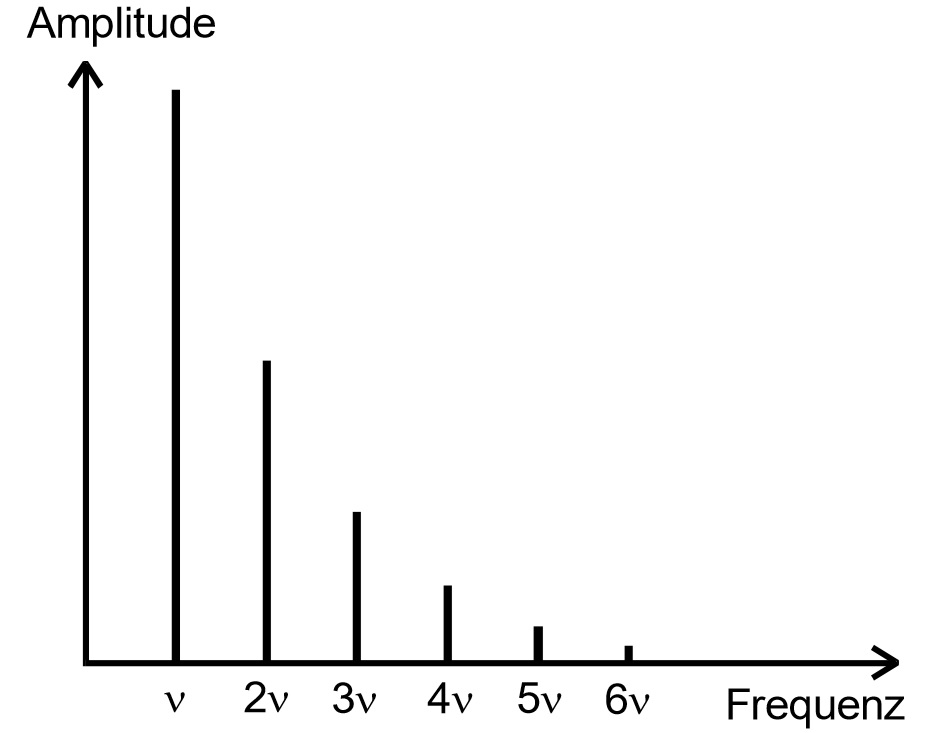
\includegraphics[width=\textwidth]{abb1.jpg}
  \caption{Ein Frequenzspektrum einer periodischen Schwingung mit der Grundfrequenz $\nu$}
  \label{fig:abb1}
\end{figure}

\subsection{Die Fourier-Transformation}
Gleichgültig ob f(t) periodisch ist oder nicht, kann man mit der Fourier-Transformation das gesamte Frequenzspektrum einer zeitabhängigen Funktion berechnen
und nicht nur die einzelnen Komponenten einer periodischen Funktion f(t) wie in \ref{eqn:gl2}.
Die Fourier-Transformation hat die Gestalt
\begin{equation}
  g(\nu) = \int_{-\infty}^{\infty} f(t) \exp{(i \nu t)} dt \label{eqn:gl3}
\end{equation}
in der $g(\nu)$ das Frequenzspektrum darstellt.
ist f(t) periodisch, dann besteht g aus einer Reihe von $\delta$-Funktionen, etwa wie in \ref{fig:abb1} angedeutet ist.
Die Fourier-Transformation ist auch umkehrbar; das bedeutete, dass die Fourier-Transformierte der Spektralfunktion g gleich der Zeitabhängigkeit des Vorganges ist
\begin{align}
  f(t) = \frac{1}{2 \pi} \int_{-\infty}^{\infty} g{\nu} \exp{(-i \nu t)} d \nu
\end{align}
Weil man über einen unendlichen Zeitraum für exakte Ergebnisse messen müsste und es in der Praxis nicht möglich ist, werden Abweichungen von den Erwartungswerten auftreten.
Durch das abschneiden der Messreihe ist die Periodizität von f aufgehoben und somit besteht g nicht aus $\delta$-Funktionen und ist überll stetig und differenzierbar.
Somit ergibt sich ein Linienspektrum mit Linien endlicher Breite.
Desweiteren werden durch das Abschneiden weitere Nebenmaxima neben den Hauptmaxima, den ursprünglichen $\delta$-Funktionen, erzeugt, deren Amplitude jedoch schnell abnimmt.\cite{AnleitungV351}

\subsection{Berechnung der Koeffizienten}
\label{sec:Koeffizienten}

Für den Versuch sollen für drei verschiedene Spannungen die Fourier-Koeffizienten berechnet werden.
Zur Vereinfachung wird angenommen, dass die Funktion entweder gerade oder ungerade ist.
Für gerade Funktionen ist $b_n = 0$, also fällt der Sinusanteil weg.
Und für ungerade Funktionen ist $a_n = 0$, also fällt der Cosinusanteil weg.
\begin{description}
  \item[Rechteckspannung]
  \begin{align*}
    a_n &= 0 \\
    b_n &= \frac{2T}{n\pi} - \frac{2T}{n\pi}(-1)^n
  \end{align*}
  \item[Sägezahnspannung]
  \begin{align*}
    a_n &= 0 \\
    b_n &= -\frac{T}{n\pi}(-1)^n
  \end{align*}
  \item[Dreieckspannung]
  \begin{align*}
    a_n &= \frac{4T}{n^2\pi^2}(-1)^n - \frac{4T}{n^2\pi^2} \\
    b_n &= 0
  \end{align*}
\end{description}
